Le jeu de données fournis contient les mesures de la qualité des
programmes couramment utilisés par les biologistes. Seize programmes
sont ainsi examinés, selon des critères tels que le nombre de lignes ou
de blocs dupliqués, le nombre et le type de warning lors de la
compilation ou encore le statut donné par valgrind sur la gestion
mémoire.

Un premier graphique nous permet de compter le nombre de programme
écrit dans chaque langage du jeu de donnée (figure \ref{prog_lang}).

% \begin{figure}[h]
%   \centering
%   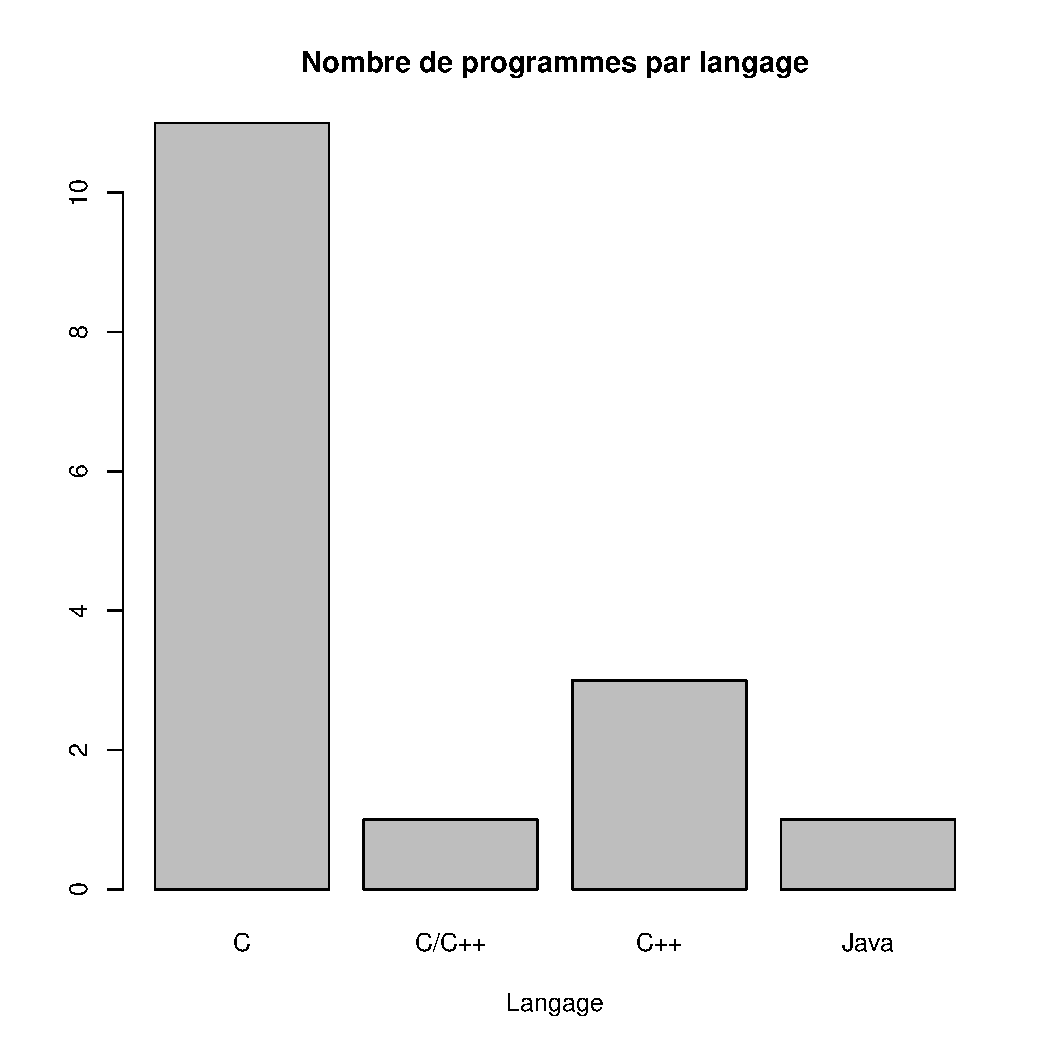
\includegraphics[width=.8\textwidth]{../figures/prog_lang.pdf}
%   \label{fig:prog_lang}
% \end{figure}

Nous avons ensuite décider de représenter le nombre de lignes de codes
dupliquées par programme (figure \ref{fig:dlin_prog}). Afin que la
représentation soit plus lisible, nous avons utilisé la commande
\lstinline{order} pour ordonner les colonnes par ordres décroissants
de valeurs. De plus, nous avons affiché les noms des programmes en
vertical, afin d'améliorer la lisibilité (grâce à l'argument
\lstinline{las = 2} de \lstinline{barplot}). Il est de plus nécessaire
de faire attention à ne pas prendre en compte les programmes pour
lesquels cette valeur n'est pas renseignée (c'est le cas de \emph{FDPPDIV}
par exemple).

% \begin{figure}[h]
%   \centering
%   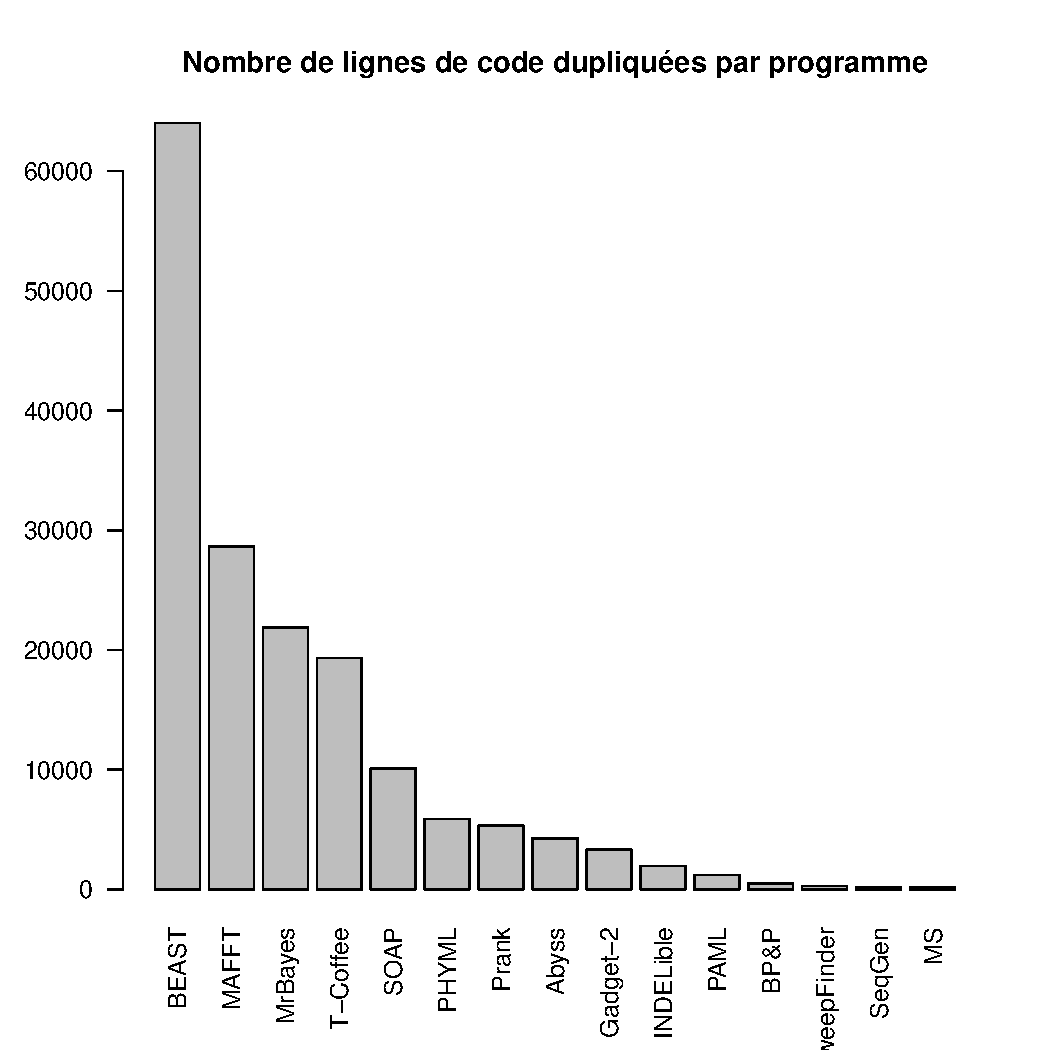
\includegraphics[width=.8\textwidth]{../figures/dlin_prog.pdf}
%   \label{fig:dlin_prog}
% \end{figure}

De même, nous avons créer un histogrammes contenant le nombre de blocs
dupliqués par programme (figure \ref{fig:dbl_prog}).

% \begin{figure}[h]
%   \centering
%   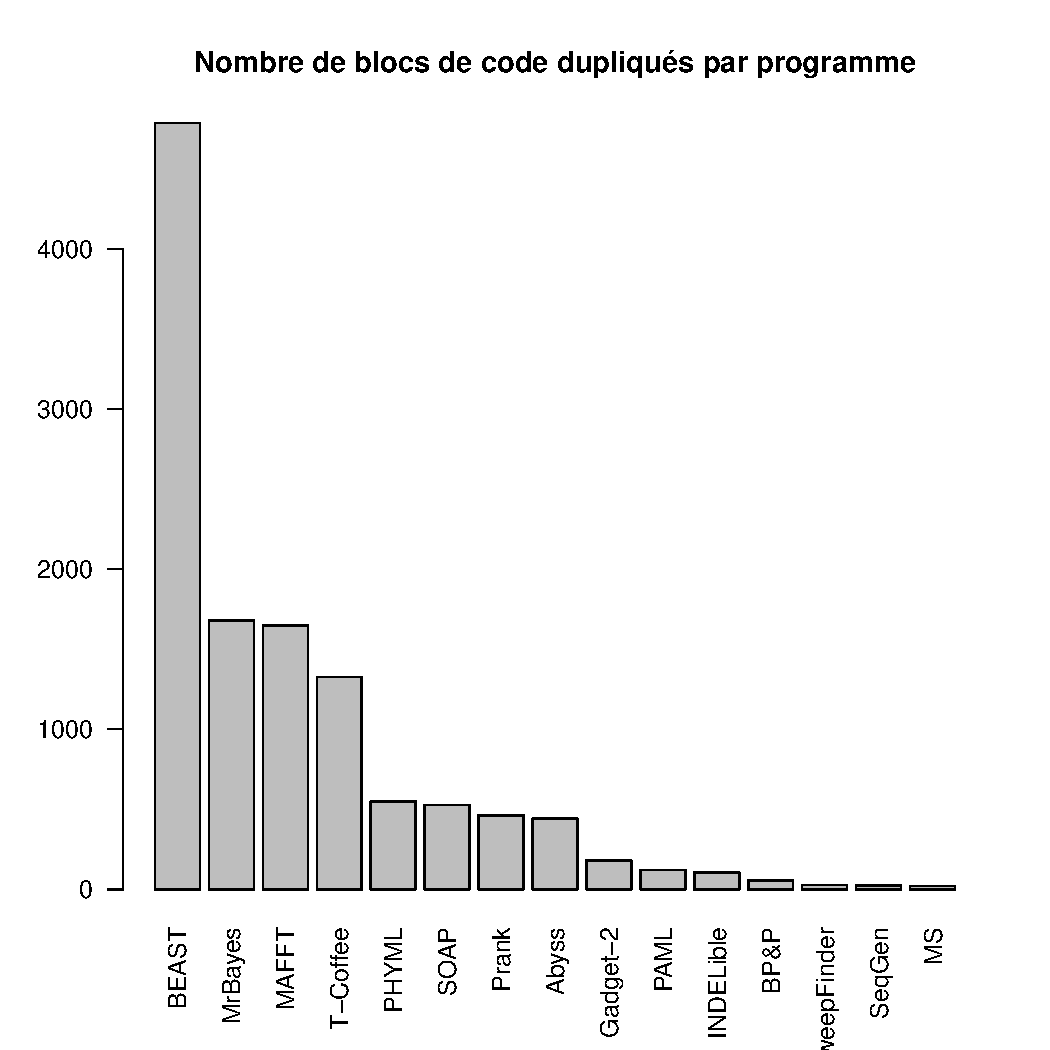
\includegraphics[width=.8\textwidth]{../figures/dbl_prog.pdf}
%   \label{fig:dbl_prog}
% \end{figure}

Enfin, nous avons généré un dernier graphique affichant le nombre de
programmes par domaine (figure \ref{fig:prog_dom}).

% \begin{figure}[h]
%   \centering
%   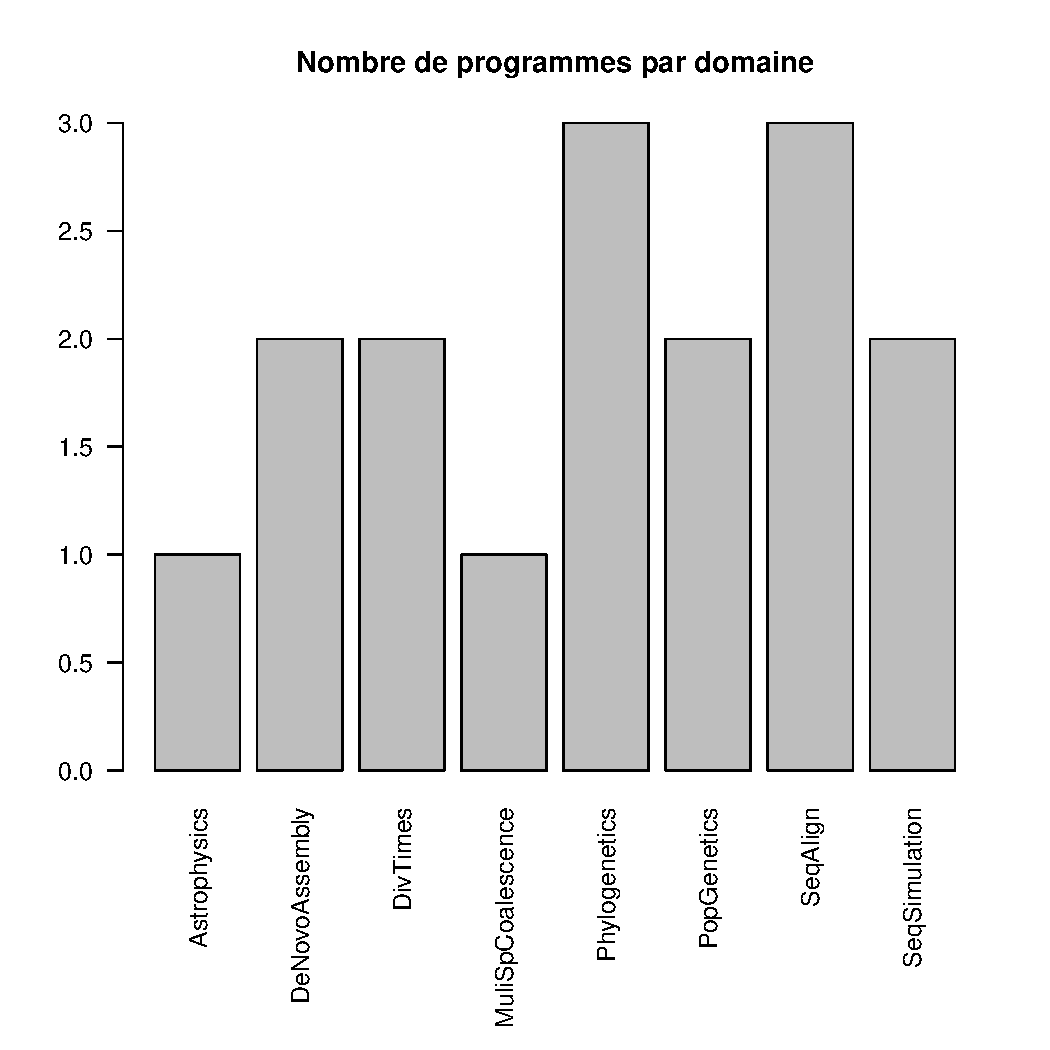
\includegraphics[width=.8\textwidth]{../figures/prog_dom.pdf}
%   \label{fig:prog_dom}
% \end{figure}
